\documentclass[addpoints]{exam}
\usepackage[utf8]{inputenc}
\usepackage[russian]{babel}
\usepackage[OT1]{fontenc}
\usepackage{amsmath}
\usepackage{amsfonts}
\usepackage{amssymb}
\usepackage{graphicx}
\usepackage{listings}
\usepackage{algorithm}
\usepackage{algpseudocode}
\usepackage{tikz}
\usetikzlibrary{matrix}
\usepackage{geometry}
 \geometry{
 a4paper,
 total={210mm,297mm},
 left=20mm,
 right=20mm,
 top=20mm,
 bottom=20mm,
 }

\newcommand{\var}[1]{{\ttfamily#1}}
\title{Все темы}
\author{Минский ШАД. Весна}

../../tasks/common/preamble.tex

\begin{document}

\maketitle

\begin{center}
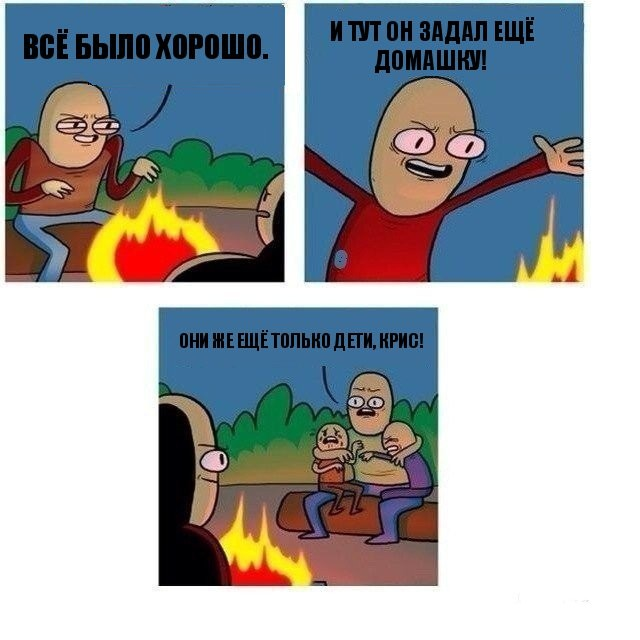
\includegraphics[scale=0.7]{homework.jpg}
\end{center}

На самом деле, как и обещалось, домашек больше не будет. Последние 10 баллов я выставлю по моему личному ощущению, как вы работали в курсе. Спасибо за участие, было весело.

\end{document}
